%---------------------
\pagestyle{plain}
\setcounter{page}{1}
\pagenumbering{arabic}
%---------------------

\chapter{مقدمه}


محوریت کار ما قرار است\cite{calcul} باشد که در آن سعی شده روش وارسی مدل با کمک نظریه تعبیر مجرد، بهبود داده شود. در\cite{clarke} روشی که معرفی شده در‌واقع ویژگی برنامه‌ها را به کمک منطق های \lr{LTL} یا \lr{CTL} بیان می‌کند. خود برنامه‌ها هم با کمک معناشناسی این منطق ها که نوع خاصی از مدل های کریپیکی به اسم سیستم گذار هستند توصیف می شوند. اما در\cite{calcul} کاری که انجام شده به این شکل است که منطق های \lr{LTL} و \lr{CTL} با عبارات منظم\cite{kleene56} جایگزین شده‌اند. علت این کار دو نکته بوده، اولی اینکه استفاده از عبارات منظم به جای منطق های نام برده شده می‌تواند برای برنامه نویسان ساده‌تر باشد و دومی اینکه عبارت منظم از از منطق های نام برده شده قدرت بیان بالاتری دارد.\cite{regisbetter} در ادامه ی کار وارسی مدل با استفاده از موجودات جدید تعریف شده به سه شکل مختلف بیان شده. در هر مرتبه بیان وارسی مدل، به‌گفته‌ی نویسنده، "ساختارمند"تر شده. می‌توان دریافت که فایده ساختارمندتر بودن بیان این است که پیاده‌سازی راحت‌تری دارد.\\
حال به بیان و بررسی تعاریف و خواص آن‌ها می‌پردازیم.


\section{روش وارسی مدل}

روش وارسی مدل یک روش صوری است که برای درستی‌یابی سیستم‌های مختلف استفاده می‌شود. در این روش معمولا ابتدا یک ماشین حالات متناهی از روی سیستم مورد بررسی ساخته می‌شود، سپس بررسی‌هایی که قرار است روی سیستم اصلی انجام شوند، روی این ماشین( مدل) انجام می‌شود. در بررسی صحت کارکرد برنامه‌های کامپیوتری از این روش استفاده می‌شود اما این تنها مورد استفاده از این روش نیست و هر منظومه‌ی دیگری که قابلیت بیان به صورت صوری را داشته باشد قابل بررسی با این روش هست. مثلا می‌توان از این روش برای بررسی صحت عملکرد برنامه‌ی قطارهای شهری استفاده کرد; در حالتی که مثلا خصوصیات مورد بررسی ما عدم رخ دادن تصادف بین قطارها یا پوشش تمام  مناطق شهر باشد. مثال های دیگر استفاده‌ی این روش در علوم کامپیوتر می تواند بررسی صحت عملکرد یک پردازنده یا مثلا الگوریتم تقسیمِ وظایف یک سیستم عامل باشد. این مثال‌ها هیچ یک برنامه‌ی کامپیوتری نیستند( هر چند که ممکن است مجبور باشیم از یک برنامه‌ی کامپیوتری برای پیاده سازی آن‌ها کمک بگیریم که در آن صورت بررسی صحت عملکرد آن برنامه‌ی کامپیوتری داستانی دیگر خواهد داشت) اما قابل بیان به صورت صوری به جای زبان طبیعی هستند.

ایده‌ی روش وارسی مدل از منطق‌های زمانی مختلف استفاده می‌کند. منطق زمانی یک نوع منطق موجهات است. منطق‌های موجهات از گسترش زبان منطق کلاسیک با اضافه کردن ادات وجهی گوناگون، با معانی متفاوتی که ممکن است در زبان طبیعی داشته باشند، ساخته می‌شوند. این ادوات غالبا در زبان طبیعی نقش قید را دارند. منطق‌های زمانی بخشی از منطق‌های موجهات هستند که به صوری‌گری ما مفهوم زمان را هم اضافه می‌کنند، یعنی قیدهایی مانند فعلا، بعدا و قبلا. منطقی که در اینجا بیان می‌کنیم \lr{LTL} نام دارد که یکی از منطق‌های زمانی است که برای روش وارسی مدل استفاده می‌شود. البته در مورد قیدهایی که نام بردیم ذکر این نکته ضروری است که در این بیانی که ما در اینجا از این منطق ارائه داده‌ایم ادوات جدید این فعل‌ها نیستند، هرچند که به کمک ادوات جدید می‌توان ادواتی برای هر یک از این قیود ساخت.
این تکه از \cite{buchi} آورده شده.

ابتدا زبان این منطق را بیان می‌کنیم و سعی می‌کنیم به طور غیر دقیق در مورد معنای فرمول‌های این زبان به خواننده یک درک شهودی بدهیم; سپس به سراغ معناشناسی صوری این منطق می‌رویم.

\subsection{زبان \lr{LTL}}
\begin{defn}
	هر عضو مجموعه‌ی $\Phi$ یک فرمول در زبان \lr{LTL} است( و $\Pi$ مجموعه‌ی فرمول‌های اتمی است و $\pi \in \Pi$):
	$$
	\Pi \subset \Phi,
	$$
	$$
	\phi \in \Phi \Leftrightarrow
	\phi ::= \pi | \phi \lor \phi |
	\neg \phi |
	\bigcirc \phi |
	\phi \mathcal{U}\phi 
$$	
	
\end{defn}
اولین نکته‌ای که برای فرمول‌های این زبان به آن نیاز داریم این است که در این منطق ما زمان را با اعداد طبیعی و هر خاصیتی که در موردشان تعریف شده نشان می‌دهیم. یعنی برای یک فرمول، زمان از عدد ۰ شروع شده و تا ابد ادامه خواهد داشت و حین گذر زمان ممکن است ارزش فرمول‌ها تغییر کند. مسلما پس از بررسی معناشناسی صوری بهتر می‌شود این مفهوم را به طور شهودی حس کرد، اما به هر حال به خواننده پیشنهاد می‌شود پیش از رسیدن به آن بخش به ادامه‌ی این بخش هم توجه شود. 

در این زبان ادوات کلاسیک 
$\neg, \lor$
هستند با همان معنایی که در منطق گزاره‌ای کلاسیک داشتند.  
در ادوات جدید 
$\bigcirc \phi$
به معنای برقرار بودن این فرمول دقیقا در لحظه‌ی بعدی( دقیقا یک لحظه) است، مثلا در شکل زیر با در نظر گرفتن اینکه در زمان 0 هستیم، این فرمول در لحظه‌ی ۱ برقرار است.
	\begin{center}
	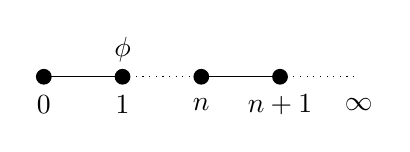
\begin{tikzpicture}
	\node at (1,0.35) (phi) {$\phi$};
	\node at (1,-0.35) (1) {$1$};
	\node at (0,-0.35) (0) {$0$};
	\node at (2,-0.35) (n) {$n$};
	\node at (3,-0.35) (1) {$n+1$};
	\node at (4,-0.35) (1) {$\infty$};
	\fill (0,0) circle (0.1cm);
	\fill (1,0) circle (0.1cm);
	\fill (2,0) circle (0.1cm);
	\fill (3,0) circle (0.1cm);
	\path (0,0) edge (1,0) 
	(1,0) edge[dotted] (2,0)
	(2,0) edge (3,0)
	(3,0) edge[dotted] (4,0);
	\end{tikzpicture}
\end{center}
$\phi \mathcal{U}\psi$
به این معنی است که فرمول سمت چپی حداقل تا قبل از اینکه فرمول سمت راستی برقرار شود، برقرار است.( مثلا اگر بگوییم "تا وقتی که باران نباریده زمین خشک است" در این صورت "زمین خشک است" به جای فرمول سمت چپ و "باران باریده است" فرمول سمت راست است).
\begin{center}
	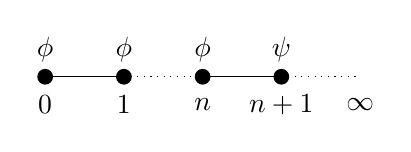
\begin{tikzpicture}
	\node at (1,0.35) (phi) {$\phi$};
	\node at (0,0.35) (phi) {$\phi$};
	\node at (2,0.35) (phi) {$\phi$};
	\node at (3,0.35) (phi) {$\psi$};
	\node at (1,-0.35) (1) {$1$};
	\node at (0,-0.35) (0) {$0$};
	\node at (2,-0.35) (n) {$n$};
	\node at (3,-0.35) (1) {$n+1$};
	\node at (4,-0.35) (1) {$\infty$};
	\fill (0,0) circle (0.1cm);
	\fill (1,0) circle (0.1cm);
	\fill (2,0) circle (0.1cm);
	\fill (3,0) circle (0.1cm);
	\path (0,0) edge (1,0) 
	(1,0) edge[dotted] (2,0)
	(2,0) edge (3,0)
	(3,0) edge[dotted] (4,0);
	\end{tikzpicture}
\end{center}

برای این زبان همان‌طور که در منطق کلاسیک از ادوات عطف و شرطی با اینکه با ادواتی که داریم قابل بیان هستند استفاده می‌کنند، ادات بیشتری هم هستند که مورد استفاده قرار می‌گیرند و با همین دو اداتی که معرفی کردیم قابل بیان هستند اما ما در اینجا از آن‌ها اسمی نیاورده‌ایم. دلیل وجود این‌ها هم راحت‌تر کردن کار کسی است که قرار است یک خاصیت را به صورت یک فرمول در این زبان بیان کند. همان طور که استفاده نکردن از یا و شرطی در منطق گزاره‌ای می‌تواند به سخت کردن بیان جملات در چارچوب این منطق منجر شود، حذف این ادوات وجهی هم بیان خواص را در این منطق مشکل می‌سازد. اما از آنجاییکه ما صرفا این بخش را برای معرفی این ایده قرار داده‌ایم، دیگر به بیان ادات وجهی دیگر نپرداخته‌ایم.

حال که به درکی شهودی از معنای فرمول‌های این زبان رسیده‌ایم، به بیان صوری این مفاهیم می‌پردازیم.

\subsection{معناشناسی \lr{LTL}}

مدل‌های این منطق را به صورت توابع
$M:\mathbb{N}_0 \rightarrow \mathit{P}(\Pi)$ 
تعریف می‌کنیم. یعنی هر مدل یک تابع است که هر عدد طبیعی را به یک مجموعه از فرمول‌های اتمی می‌برد. این در واقع قرار است به این معنی باشد که یک مدل به تعبیری به این معنی است که در هر لحظه کدام یک از فرمول‌های اتمی درست هستند. مثلا در مدلی به نام $M_i$ در واقع
$M_i(5)$
مجموعه‌ی اتم‌هایی است که در لحظه‌ی 5 طبق این مدل درست هستند و اگر اتمی در این مجموعه نباشد ارزش غلط دارد.
درستی یک فرمول در یک مدل را با 
$M,i$
نشان می‌دهیم و 
$M,i \models \phi$
به این معنی است که در لحظه‌ی $i$در مدل $\phi$ ارزش درست دارد. این مفهوم را به صورت بازگشتی به شکل زیر تعریف می‌کنیم:


\begin{flushleft}
$	M,i \models \pi \:\:\: \mathit{iff} \:\:\: \pi \in M(i)$\\
$	M,i \models \neg \phi \:\:\: \mathit{iff} \:\:\: M,i\nvDash \phi$\\
$	M,i \models \phi \lor \psi \:\:\: \mathit{iff} \:\:\: M,i \models \phi \:\:\: \mathit{or} \:\:\: M,i \models \psi$\\
	 $M,i \models \bigcirc \phi  \:\:\:  \mathit{iff} \:\:\: M,i+1 \models \phi$\\
	 $M,i \models \phi \mathcal{U} \psi \:\:\: \mathit{iff} \:\:\: 
	 \exists k \geq i \in \mathbb{N}_0: \forall i\leq j< k: M,j \models \phi \:\:\: \mathit{and} \:\:\: M,k \models \psi$
\end{flushleft}

برای یک فرمول اگر مدلی وجود داشته باشد که در آن مدل آن فرمول صادق باشد، آنگاه آن فرمول را \emph{ارضاپذیر} می‌گوییم. اگر یک فرمول در هر مدلی صادق باشد، آن فرمول را \emph{معتبر} می‌گوییم.\\
شیوه‌ی دیگری برای بیان همین معناشناسی که گفتیم به شکل اتوماتا است. 


\section{نظریه تعبیر مجرد}




\chapter{برخی مفاهیم اولیه}


\section{نحو زبان مورد بررسی‬}

زبان بیان برنامه ها زیرمجموعه ای از دستورات زبان \lr{C} است، به شکل زیر:
$$\mathsf{x,y},... \in \mathbb{X}\hspace{4.65cm}$$
$$\mathsf{A} \in \mathbb{A} ::=\mathsf{1\:|\:x\:|\:A_1 - A_2\hspace{2.4cm}}$$  
$$\mathsf{B \in \mathbb{B} ::=A_1<A_2 \:|\: B_1 \: nand\: B_2\hspace{1.2cm}}$$
$$\mathsf{E \in \mathbb{E}::= A \: | \: B\hspace{4cm}}$$
$$\mathsf{S\in \mathbb{S} ::=\hspace{5cm}  }$$
$$\mathsf{x\doteq A; \hspace{2.25cm}}$$
$$\mathsf{|\:\:\:;\hspace{3.75cm}}$$
$$\mathsf{|\:\:\:if\:(B)\:S\:|\:if\:(B)\:S\:else\:S}$$
$$\mathsf{|\:\:\:while\:(B)\:S\: | \: break;\hspace{0.65cm}}$$
$$\mathsf{|\:\:\:\{Sl\}\hspace{3.15cm}}$$
$$\mathsf{Sl \in \mathbb{SL}::=Sl\:\:\:S\:|\:\backepsilon}\hspace{3.05cm}$$
$$\mathsf{P\in \mathbb{P}\:::=Sl}\hspace{4.25cm}$$

\vspace{1cm}
در اینجا زیر مجموعه‌ای از دستورات زبان \lr{C} را داریم. همین‌طور که قابل مشاهده است این زبان تا حد ممکن کوچک شده. علت این کار را بعدا عمیق‌تر حس خواهیم‌کرد. علتْ ساده‌تر شدن کار برای ارائه‌ی معناشناسی و تعبیر مجرد آن است. در اینجا راحتی آن برنامه‌نویسی که قرار است با این زبان برنامه بنویسد مطرح نبوده چون اصلا این زبان برای این کار ساخته نشده. نویسنده‌ی \cite{calcul} در اینجا صرفا می‌خواسته فرآیند را نشان دهد. اگر به فرض برای زبانی مانند پایتون بخواهیم درستی‌یابی با استفاده از روش ارائه شده را درست کینم، می‌توانیم همه‌ی راهی که در \cite{calcul} برای زبان توصیف شده، رفته‌شده را برای پایتون هم برویم و به یک تحلیل‌گر ایستا برای پایتون برسیم.
در مورد قدرت بیان این زبان هم می‌توانیم بگوییم که می‌توانیم باقی اعداد را از روی عدد ۱ و عملگر منها بسازیم. مثلا ابتدا 0 را به کمک ۱-۱ می سازیم و سپس با استفاده از 0 می‌توانیم یکی یکی اعداد منفی را بسازیم و سپس بعد از آن به سراغ اعداد مثبت می‌رویم که با کمک 0 و هر عدد منفی‌ای که ساختیم، ساخته می شوند. باقی اعداد و حتی باقی عملگر‌ها( یعنی به غیر از اعداد طبیعی) نیز از روی آنچه داریم قابل‌ساختن است. در مورد عبارت‌های بولی نیز داستان به همین منوال است. یعنی اینجا صرفا ادات شفر تعریف شده و باقی عملگر‌های بولی را می‌توان با استفاده از همین عملگر ساخت. باقی دستورات نیز دستورات شرط و حلقه هستند. باقی دستورات قرار است مطابق چیزی که از زبان \lr{C} انتظار داریم کار بکنند. در مورد دستور \lr{$\mathsf{break;}$} ذکر این نکته ضروری است که اجرای آن قرار است اجرای برنامه را از دستوری بعد از داخلی‌ترین حلقه‌ای که \lr{$\mathsf{break;}$} داخلش قرار دارد ادامه ‌دهد. در پایان می توان ثابت کرد که این زبان هم قدرت با مدل دیویس\cite{davis} است. 
توجه داریم که هر‌چه در این بخش در‌مورد معنای دستورات این زبان گفتیم، به هیچ وجه صوری نبود و صرفا درک شهودی ای که از معنای اجرای هر‌یک از دستورات داشتیم را بیان کردیم. بیان صوری معنای برنامه‌ها را، که برخلاف درک شهودی‌مان قابل انتقال به کامپیوتر‌ است، در ادامه بیان خواهیم‌کرد. طبیعتا این بیان صوری از روی یک درک شهودی ساخته شده‌است.

\section{معناشناسی زبان مورد بررسی‬}
معناشناسی زبانی را که در بخش پیش آوردیم با کمک مفاهیمی به نام برچسب و رد پیشوندی و عملگر چسباندن روی دو رود پیشوندی مختلف تعریف خواهیم‌کرد و نام این معناشناسی نیز معناشناسی رد پیشوندی است.\\

\subsection{برچسب‌ها}

با‌وجود اینکه خود زبان \lr{C} در قسمتی از زبان خود چیز‌هایی به نام برچسب دارد اما همین‌طور که در بخش پیشین دیدیم، در زبانی که اینجا در حال بحث روی آن هستیم خبری از برچسب‌ها نیست. اما برای تعریف صوری معنای برنامه‌ها، به شکلی که مورد بحث است، به آن‌ها نیاز است. در این بخش ابتدا به توضیحی مختصر در مورد برچسب‌ها در معناشناسی‌ زبان مورد بحث می‌پردازیم. تعاریف صوری دقیق این موجودات در پیوست \cite{calcul} آورده‌شده‌اند. از آوردن مستقیم این تعاریف در اینجا خود‌داری کرده‌ایم. البته در مورد معنای صوری برجسب‌ها هم ذکر این نکته ضروری است که نویسنده‌ی \cite{calcul} حتی به صورت صوری هم برای هر بخش از برنامه این کار را به طور دقیق انجام نداده و انجام این کار به طور دقیق‌تر را احتمالا به کسی که قرار است یک پیاده سازی کامل از این روش داشته باشد سپرده.


در زبانمان \lr{$\mathsf{S}$}ها بخشی از موجودات موجود در زبان هستند. برچسب ها را برای \lr{$\mathsf{S}$}ها تعریف می‌کنیم. برچسب‌ها با کمک توابع \lr{labs, in, brks-of, brk-to, esc, aft, at} تعریف می‌شوند. در‌واقع هر $\mathsf{S}$ به ازای بعضی از این توابع یک برجسب دارد و این‌ها در‌واقع نشان‌دهنده‌ی آن برچسب هستند. بعض دیگر این توابع برای هر $\mathsf{S}$ ممکن است یک مجموعه از برچسب‌ها را تعیین‌ کند و یکی از آن‌ها هم با گرفتن $\mathsf{S}$ یک مقدار بولی را بر‌می‌گرداند. 
\\\\
\lr{at$\llbracket\mathsf{S}\rrbracket$} : برچسب شروع $\mathsf{S}$.\\
\lr{aft$\llbracket\mathsf{S}\rrbracket$} : برچسب پایان $\mathsf{S}$، اگر پایانی داشته باشد.\\
\lr{esc$\llbracket\mathsf{S}\rrbracket$} : یک مقدار بولی را باز‌‌می‌گرداند که بسته به اینکه در $\mathsf{S}$ دستور $\mathsf{break;}$ وجود دارد یا خیر، مقدار درست یا غلط را بر‌می‌گرداند.\\
\lr{brk-to$\llbracket\mathsf{S}\rrbracket$} : برچسبی است که اگر حین $\mathsf{S}$ دستور $\mathsf{break;}$ اجرا شود، برنامه از آن نقطه ادامه پیدا می کند.\\
\lr{brks-of$\llbracket\mathsf{S}\rrbracket$} : مجموعه‌ای از برچسب $\mathsf{break;}$ های $\mathsf{S}$ را بر‌می‌گرداند.\\
\lr{in$\llbracket\mathsf{S}\rrbracket$} : مجموعه‌ای از تمام برچسب‌های درون $\mathsf{S}$ را برمی‌گرداند.\\
\lr{labs$\llbracket\mathsf{S}\rrbracket$} : مجموعه‌ای از تمام بر‌چسب‌هایی که با اجرای $\mathsf{S}$ قابل دسترسی هستند را بر‌می‌گرداند.\\\\\\


\subsection{رد پیشوندی}


پس از تعریف برچسب‌ها به سراغ تعریف رد پیشوندی می‌رویم. پیش از آن باید وضعیت‌ها و محیط‌ها را تعریف کنیم.
\begin{defn}
	(محیط): به ازای مجموعه مقادیر $\mathbb{V}$ و مجموعه متغیرهای $\mathbb{X}$ تابع 
	$\rho : \mathbb{X} \rightarrow \mathbb{V}$ 
	را یک محیط می‌گوییم. مجموعه‌ی همه‌ی محیط‌ها را با $\mathbb{EV}$ نمایش می‌دهیم.
\end{defn}

\begin{defn}
	(وضعیت): به هر زوج مرتبْ به ترتیب متشکل از یک برچسب $l$ و یک محیط $\rho$ یک وضعیت (یا حالت)  
	$\langle l , \rho \rangle$
	می‌گوییم. مجموعه‌ی همه‌ی وضعیت‌ها را با $\mathfrak{S}$ نشان می‌دهیم.
\end{defn}
\begin{defn}
	(رد پیشوندی): به یک دنباله از وضعیت‌ها(با امکان تهی بودن) یک رد پیشوندی می‌گوییم.
\end{defn}

هر رد پیشوندی یک دنباله است که قرار است توصیفی از چگونگی اجرای برنامه باشد. وضعیت‌ها همان‌طور که از نامشان پیداست قرار‌ است موقعیت لحظه‌ای برنامه را توصیف کنند. $l$ قرار است برچسب برنامه‌ی در حال اجرا باشد و $\rho$ مقدار متغیر‌ها را در آن موقع از اجرای برنامه نشان می‌دهد. دنباله‌های ما می‌توانند متناهی یا نامتناهی باشند. مجموعه‌ی ردهای پیشوندی‌ متناهی را با $\mathfrak{S^+}$ و مجموعه‌ی ردهای پیشوندی نامتناهی را با  $\mathfrak{S^\infty}$ نمایش می‌دهیم. مجموعه‌ی همه‌ی ردهای پیشوندی را هم با $\mathfrak{S^{+\infty}}$ نمایش می‌دهیم. 
با‌توجه به آنچه گفتیم، یک عملگر چسباندن $\Join$ را روی ردهای پیشوندی تعریف می‌کنیم. 
\begin{defn}
	(عملگر چسباندن): اگر داشته باشیم 
	$\pi_1 , \pi_2 \in \mathfrak{S^{+\infty}}  , \sigma_1 ,\sigma_2 \in \mathfrak{S}$
	داریم:\\
	\begin{center}
		اگر $\pi_1 \in \mathfrak{S^+} $ داریم  $\hspace{2.60cm}  $                                     
		$\pi_1 \Join \pi_2 = \pi_1$    \\
		اگر $\sigma_1\neq\sigma_2$    $\hspace{1.6cm}  $
		$\pi_1 \Join \pi_2$ تعریف نشده است
		\\اگر $\pi_1 \in \mathfrak{S^\infty} $ داریم   $\hspace{1cm}  $ 
		$\pi_1 \sigma_1 \Join \sigma_1 \pi_2 = \pi_1 \sigma_1 \pi_2 $
		
	\end{center}
\end{defn}
همینطور $\epsilon$ هم یک رد پیشوندی است که حاوی هیچ وضعیتی نیست. به عبارت دیگر یک دنباله‌ی تهی است.

\subsection{تعریف صوری معناشناسی رد پیشوندی}
در این بخش قرار است دو تابع $\mathcal{A}$ و $\mathcal{B}$ را به ترتیب روی عبارات حسابی و بولی زبانمان یعنی $\mathsf{A}$ها و $\mathsf{B}$ها تعریف کنیم سپس با کمک آنها $\mathcal{S^*}$ را روی  مجموعه‌ای از اجتماع معنای $\mathsf{S}$ها و $\mathsf{Sl}$ها تعریف می کنیم. پس در نهایت هدف ما تعریف  $\mathcal{S^*}$ است.


\begin{defn}
	(معنای عبارات حسابی - تابع $\mathcal{A}$): تابع 
	$\mathcal{A}:\mathbb{A}\rightarrow \mathbb{EV} \rightarrow \mathbb{V}$
	را به صورت بازگشتی روی ساختار 
	$\mathsf{A} \in \mathbb{A}$
	به شکل زیر تعریف می‌کنیم:
	$$\mathcal{A\llbracket\mathsf{1}\rrbracket\rho = }1     $$
	$$\mathcal{A\llbracket\mathsf{x}\rrbracket\rho = } \rho(\mathsf{x})          $$
	$$\mathcal{A\llbracket\mathsf{A_1-A_2}\rrbracket\rho = }\mathcal{A\llbracket\mathsf{A_1}\rrbracket\rho }- \mathcal{A\llbracket\mathsf{A_2}\rrbracket\rho }       $$
	
\end{defn}

\begin{defn}
	(معنای عبارات بولی - تابع $\mathcal{B}$): تابع 
	$\mathcal{B}: \mathbb{B} \rightarrow \mathbb{EV} \rightarrow \mathbb{BOOL}$
	را به صورت بازگشتی روی ساختار 
	$\mathsf{B} \in \mathbb{B}$
	به شکل زیر تعریف می‌کنیم:
	
	\begin{center}
		اگر $\mathcal{A\llbracket\mathsf{A_1}\rrbracket\rho }$ کوچکتر از $\mathcal{A\llbracket\mathsf{A_2}\rrbracket\rho }$ باشد
		$\mathcal{B\llbracket\mathsf{A_1<A_2}\rrbracket\rho = } True   \hspace{2cm}  $\\
		اگر $\mathcal{A\llbracket\mathsf{A_1}\rrbracket\rho }$ بزرگتر از $\mathcal{A\llbracket\mathsf{A_2}\rrbracket\rho }$ باشد
		$\mathcal{B\llbracket\mathsf{A_1<A_2}\rrbracket\rho = } False   \hspace{2cm}  $\\
		$ \mathcal{B\llbracket\mathsf{B_1 nand B_2}\rrbracket\rho = } \neg(\mathcal{B\llbracket\mathsf{B_1}\rrbracket\rho}   \wedge \mathcal{B\llbracket\mathsf{B_2}\rrbracket\rho}) $
	\end{center}
\end{defn}

طبعا $\wedge$ و $\neg$ در فرازبان هستند.\\\\
در ادامه به تعریف $\mathcal{S^*}$ می‌پردازیم. این کار را با تعریف $\mathcal{S^*}$ روی هر ساخت $\mathsf{S}$ و $\mathsf{Sl}$ انجام می‌دهیم.
پیش از ادامه‌ی بحث باید این نکته را در‌مورد علامت‌گذاری‌هایمان ذکر کنیم که منظور از $        \mathsf{S} ::= l \mathsf{break;}  $ این است که تاکید کرده‌ایم که $\mathsf{S}$ با برچسب $l$ شروع شده‌است وگرنه همین طور که گفتیم   $l$ جزو زبان نیست.\\\\

\begin{defn}
	(معنای برنامه‌ها - تابع $\mathcal{S}^*$): 
	اگر $        \mathsf{S} ::= \mathsf{break;}  $ باشد، ردهای پیشوندی متناظر با اجرای این دستور را به شکل مجموعه‌ی زیر تعریف می کنیم:
	$$\mathcal{S^*} \llbracket\mathsf{S}\rrbracket = \{ \langle at\llbracket\mathsf{S}\rrbracket , \rho \rangle | \rho \in \mathbb{EV}       \} \cup     \{ \langle at\llbracket\mathsf{S}\rrbracket , \rho \rangle \langle brk-to\llbracket\mathsf{S}\rrbracket , \rho \rangle | \rho \in \mathbb{EV}       \}             $$   
	
	
	اگر $        \mathsf{S} ::=  \mathsf{x\doteq A;}  $ باشد، ردهای پیشوندی متناظر با اجرای این دستور را به شکل مجموعه‌ی زیر تعریف می کنیم:
	$$\mathcal{S^*} \llbracket\mathsf{S}\rrbracket = \{ \langle at\llbracket\mathsf{S}\rrbracket , \rho \rangle | \rho \in \mathbb{EV}       \} \cup     \{ \langle at\llbracket\mathsf{S}\rrbracket , \rho \rangle \langle aft\llbracket\mathsf{S}\rrbracket , \rho[\mathsf{x}\leftarrow \mathcal{A}\llbracket\mathsf{A}\rrbracket\rho] \rangle | \rho \in \mathbb{EV}       \}             $$   
	
	اگر $         \mathsf{S} ::= \mathsf{if}  \mathsf{ (B) S_t}  $ باشد، ردهای پیشوندی متناظر با اجرای این دستور را به شکل مجموعه‌ی زیر تعریف می کنیم:
	$$\mathcal{S^*} \llbracket\mathsf{S}\rrbracket = \{ \langle at\llbracket\mathsf{S}\rrbracket , \rho \rangle | \rho \in \mathbb{EV}       \} \cup     \{ \langle at\llbracket\mathsf{S}\rrbracket , \rho \rangle \langle aft\llbracket\mathsf{S}\rrbracket , \rho \rangle | \mathcal{B}\llbracket\mathsf{B}\rrbracket \rho =False      \} 
	$$$$\cup    \{ \langle at\llbracket\mathsf{S}\rrbracket , \rho \rangle \langle at\llbracket\mathsf{S_t}\rrbracket , \rho \rangle 
	\pi | \mathcal{B}\llbracket\mathsf{B}\rrbracket \rho =True  \wedge   \langle  at\llbracket\mathsf{S_t}\rrbracket  , \rho \rangle \pi \in \mathcal{S} \llbracket\mathsf{S_t}\rrbracket    \}          $$ 
	
	
	اگر $         \mathsf{S} ::= \mathsf{if}  \mathsf{ (B) S_t else S_f}  $ باشد، ردهای پیشوندی متناظر با اجرای این دستور را به شکل مجموعه‌ی زیر تعریف می کنیم:
	$$\mathcal{S} \llbracket\mathsf{S}\rrbracket = \{ \langle at\llbracket\mathsf{S}\rrbracket , \rho \rangle | \rho \in \mathbb{EV}       \} $$$$\cup     \{ \langle at\llbracket\mathsf{S}\rrbracket , \rho \rangle \langle at\llbracket\mathsf{S_f}\rrbracket , \rho \rangle 
	\pi | \mathcal{B}\llbracket\mathsf{B}\rrbracket \rho =False  \wedge   \langle  at\llbracket\mathsf{S_f}\rrbracket  , \rho \rangle \pi \in \mathcal{S} \llbracket\mathsf{S_f}\rrbracket    \}  
	$$$$\cup    \{ \langle at\llbracket\mathsf{S}\rrbracket , \rho \rangle \langle at\llbracket\mathsf{S_t}\rrbracket , \rho \rangle 
	\pi | \mathcal{B}\llbracket\mathsf{B}\rrbracket \rho =True  \wedge   \langle  at\llbracket\mathsf{S_t}\rrbracket  , \rho \rangle \pi \in \mathcal{S} \llbracket\mathsf{S_t}\rrbracket    \}          $$ \\
	
	
	اگر 
	$         \mathsf{Sl} ::= \backepsilon  $
	باشد، ردهای پیشوندی متناظر با اجرای این دستور را به شکل مجموعه‌ی زیر تعریف می کنیم:
	
	$$\mathcal{S} \llbracket\mathsf{Sl}\rrbracket = \{ \langle at\llbracket\mathsf{Sl}\rrbracket , \rho \rangle | \rho \in \mathbb{EV}       \}        $$ \\
	
	اگر $         \mathsf{Sl} ::= \mathsf{Sl' \:\:\: S}  $ باشد، ردهای پیشوندی متناظر با اجرای این دستور را به شکل مجموعه‌ی زیر تعریف می کنیم:
	$$\mathcal{S} \llbracket\mathsf{Sl}\rrbracket = \mathcal{S} \llbracket\mathsf{Sl'}\rrbracket \cup( \mathcal{S} \llbracket\mathsf{Sl'}\rrbracket
	\Join \mathcal{S} \llbracket\mathsf{S}\rrbracket )      $$ \\
	
	
	
	اگر $         \mathsf{S} ::= \mathsf{while (B)S_b }   $ باشد، ماجرا نسبت به حالات قبل اندکی پیچیده‌تر می‌شود. تابعی به اسم $\mathcal{F} $ را تعریف خواهیم‌کرد که در حقیت دو ورودی دارد. ورودی اول آن یک دستور حلقه است و ورودی دوم آن یک مجموعه. به عبارتی دیگر می‌توانیم بگوییم به ازای هر حلقه یک تابع $\mathcal{F} $  جداگانه تعریف می‌شود که مجموعه‌ای از ردهای پیشوندی را می گیرد و مجموعه‌ای دیگر از همین موجودات را بازمی‌گرداند. کاری که این تابع قرار است انجام دهد این است که انگار یک دور دستورات داخل حلقه را اجرا می کند و دنباله‌هایی جدید را از دنباله‌های قبلی می‌سازد. معنای یک حلقه را کوچکترین نقطه ثابت این تابع در نظر می‌گیریم. در ادامه تعریف $\mathcal{F} $ آمده. با دیدن تعریف می توان به دلیل این کار پی‌برد. آن نقطه‌ای که دیگر $\mathcal{F} $ روی آن اثر نمی‌کند یا حالتی است که در آن دیگر شرط حلقه برقرار نیست و اصولا قرار نیست دستورات داخل حلقه اجرا شوند که طبق تعریف $\mathcal{F} $  می‌توانیم ببینیم که $\mathcal{F} $  در این حالت چیزی به ردهای پیشوندی اضافه نمی‌کند. یا اینکه حلقه به دستور $\mathsf{break;}$ خورده که در آن صورت وضعیتی به ته ردهای پیشوندی اضافه می‌شود که برچسبش خارج از مجموعه برچسب دستورات حلقه است و همین اضافه کردن هر چیزی را به ته ردهای پیشوندی موجود، توسط $\mathcal{F} $  غیرممکن می‌کند. بنابراین نقطه ثابت مفهوم مناسبی است برای اینکه از آن در تعریف صوری معنای حلقه استفاده کنیم. علت اینکه کوچکترین نقطه ثابت را به عنوان معنای حلقه در نظر می‌گیریم هم این است که مطمئن هستیم کوچکترین نقطه ثابت، هر رد پیشوندی ای را در خود داشته باشد به معنای اجرای برنامه مرتبط است. برای درک بهتر این نکته می‌توان به این نکته توجه کرد که با اضافه کردن وضعیت‌هایی کاملا بی‌ربط به اجرای برنامه به ته رد‌های پیشوندی، که صرفا برچسب متفاوتی با آخرین وضعیت هر رد پیشوندی دارند، نقطه ثابت جدیدی ساخته ایم. پس اگر خودمان را محدود به انتخاب کوچکترین نقطه ثابت نکنیم، به توصیفات صوری خوبی از برنامه‌ها دست پیدا نخواهیم‌کرد. در مورد نقطه ثابت تنها این نکته باقی می‌ماند که اصلا از کجا می‌دانیم که چنین نقطه ثابتی وجود دارد که در این صورت باید گفت مجموعه‌هایی که از ردهای پیشوندی تشکیل می‌شوند با عملگر زیرمجموعه بودن یک مشبکه را تشکیل می‌دهند و بنا به قضیه تارسکی\cite{tarski} برای چنین موجودی نقطه ثابت وجود دارد.
	تعاریف موجوداتی که درموردشان صحبت کردیم به این شکل است:
	
	$$\mathcal{S} \llbracket\mathsf{S}\rrbracket = lfp^{\subseteq}\: \mathcal{F\llbracket\mathsf{S}\rrbracket}      $$ $$\mathcal{F} \llbracket\mathsf{S}\rrbracket X= \{ \langle at\llbracket\mathsf{S}\rrbracket , \rho \rangle | \rho \in \mathbb{EV}       \} \cup $$
	$$  \{ \pi_2 \langle l ,\rho \rangle \langle aft\llbracket\mathsf{S}\rrbracket,\rho \rangle |  \pi_2 \langle l ,\rho \rangle \in X \wedge \mathcal{B}\llbracket\mathsf{B}\rrbracket\rho=False \wedge l= at\llbracket\mathsf{S}\rrbracket   \} \cup      $$
	$$  \{ \pi_2 \langle l ,\rho \rangle \langle at\llbracket\mathsf{S_b}\rrbracket,\rho \rangle \pi_3 |  \pi_2 \langle l ,\rho \rangle \in X \wedge \mathcal{B}\llbracket\mathsf{B}\rrbracket\rho=True \wedge$$$$  \langle at\llbracket\mathsf{S_b}\rrbracket,\rho \rangle \pi_3 \in  \mathcal{S} \llbracket\mathsf{S_b}\rrbracket   \wedge   l= at\llbracket\mathsf{S}\rrbracket  \}  $$\\
	
	اگر $         \mathsf{S} ::=;  $ باشد، ردهای پیشوندی متناظر با اجرای این دستور را به شکل مجموعه‌ی زیر تعریف می کنیم:
	$$\mathcal{S} \llbracket\mathsf{S}\rrbracket = \{ \langle at\llbracket\mathsf{S}\rrbracket , \rho \rangle | \rho \in \mathbb{EV}       \} \cup     \{ \langle at\llbracket\mathsf{S}\rrbracket , \rho \rangle \langle aft\llbracket\mathsf{S}\rrbracket , \rho \rangle | \rho \in \mathbb{EV}       \}             $$  
	
	
	اگر $         \mathsf{S} ::=\{\mathsf{Sl}\}  $ باشد، ردهای پیشوندی متناظر با اجرای این دستور را به شکل مجموعه‌ی زیر تعریف می کنیم:
	$$\mathcal{S} \llbracket\mathsf{S}\rrbracket = \mathcal{S} \llbracket\mathsf{Sl}\rrbracket $$   \\
\end{defn}







